% Figure from MATH 591 notes, section 67 (local existence of integral curves: the board cartoon). From the board (Lecture 23 delivery).
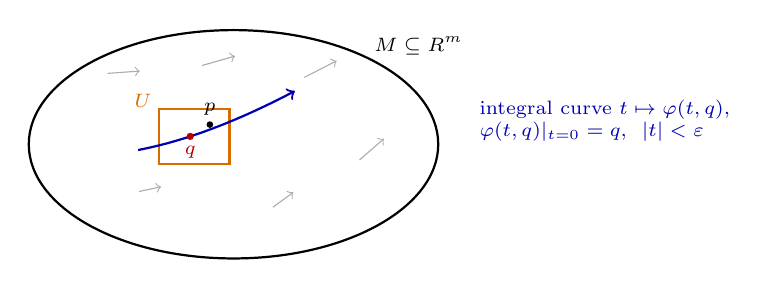
\begin{tikzpicture}[scale=1.0]
\draw[thick] (0,0) ellipse (2.6 and 1.45); \node[font=\scriptsize] at (2.35,1.25) {$M \subseteq \mathbb{R}^m$};
\draw[->, gray!65] (-1.60,0.90) -- (-1.19,0.93);
\draw[->, gray!65] (-0.40,1.00) -- (0.02,1.12);
\draw[->, gray!65] (0.90,0.85) -- (1.31,1.06);
\draw[->, gray!65] (1.60,-0.20) -- (1.91,0.07);
\draw[->, gray!65] (0.50,-0.80) -- (0.76,-0.61);
\draw[->, gray!65] (-1.20,-0.60) -- (-0.92,-0.54);
\draw[orange!85!black, thick] (-0.95,-0.25) rectangle (-0.05,0.45); \node[orange!85!black, font=\scriptsize] at (-1.15,0.55) {$U$};
\fill (-0.3,0.25) circle (1.2pt) node[above, font=\scriptsize] {$p$};
\draw[blue!70!black, thick, ->] plot[smooth] coordinates {(-1.211,-0.073) (-1.200,-0.071) (-1.189,-0.069) (-1.179,-0.066) (-1.168,-0.064) (-1.157,-0.062) (-1.146,-0.060) (-1.135,-0.058) (-1.125,-0.055) (-1.114,-0.053) (-1.103,-0.051) (-1.092,-0.048) (-1.081,-0.046) (-1.070,-0.043) (-1.059,-0.041) (-1.049,-0.039) (-1.038,-0.036) (-1.027,-0.033) (-1.016,-0.031) (-1.005,-0.028) (-0.994,-0.026) (-0.983,-0.023) (-0.972,-0.020) (-0.961,-0.018) (-0.950,-0.015) (-0.939,-0.012) (-0.928,-0.010) (-0.917,-0.007) (-0.906,-0.004) (-0.895,-0.001) (-0.884,0.002) (-0.873,0.005) (-0.862,0.007) (-0.851,0.010) (-0.840,0.013) (-0.829,0.016) (-0.818,0.019) (-0.807,0.022) (-0.796,0.026) (-0.785,0.029) (-0.774,0.032) (-0.763,0.035) (-0.752,0.038) (-0.741,0.041) (-0.729,0.045) (-0.718,0.048) (-0.707,0.051) (-0.696,0.054) (-0.685,0.058) (-0.674,0.061) (-0.662,0.065) (-0.651,0.068) (-0.640,0.071) (-0.629,0.075) (-0.618,0.078) (-0.606,0.082) (-0.595,0.085) (-0.584,0.089) (-0.573,0.093) (-0.561,0.096) (-0.550,0.100) (-0.529,0.107) (-0.508,0.114) (-0.488,0.121) (-0.467,0.128) (-0.446,0.135) (-0.425,0.142) (-0.404,0.149) (-0.383,0.157) (-0.362,0.164) (-0.341,0.172) (-0.320,0.180) (-0.299,0.188) (-0.277,0.195) (-0.256,0.203) (-0.235,0.212) (-0.213,0.220) (-0.192,0.228) (-0.171,0.236) (-0.149,0.245) (-0.128,0.253) (-0.106,0.262) (-0.084,0.271) (-0.063,0.280) (-0.041,0.289) (-0.019,0.298) (0.003,0.307) (0.025,0.316) (0.046,0.325) (0.068,0.335) (0.090,0.344) (0.113,0.354) (0.135,0.364) (0.157,0.373) (0.179,0.383) (0.201,0.393) (0.224,0.403) (0.246,0.414) (0.269,0.424) (0.291,0.434) (0.314,0.445) (0.336,0.455) (0.359,0.466) (0.382,0.477) (0.405,0.488) (0.428,0.499) (0.451,0.510) (0.474,0.521) (0.497,0.532) (0.520,0.544) (0.543,0.555) (0.566,0.567) (0.589,0.579) (0.613,0.590) (0.636,0.602) (0.660,0.614) (0.683,0.626) (0.707,0.639) (0.731,0.651) (0.755,0.663) (0.778,0.676)};
\fill[red!70!black] (-0.55,0.1) circle (1.3pt) node[below, font=\scriptsize] {$q$};
\node[blue!70!black, font=\scriptsize, anchor=west, align=left] at (3.0,0.3) {integral curve $t \mapsto \varphi(t, q)$,\\ $\varphi(t,q)|_{t=0} = q$, \ $|t| < \varepsilon$};
\end{tikzpicture}
